\chapter{Введение}
\section{Экспериментальные данные по изучению грязных сверхпроводников}
Стандартной картиной поведения чистых сверхпроводников с тривиальным спариванием является следующий (интересующий нас) набор качественных свойств \cite{deZhen}:
\begin{itemize}
	\item наличие температуры перехода $T_c$, характеризующей пропадание электрического сопротивления при $T < T_c$; соответствующее состояние называется сверхпроводящим;
	\item при температурах гораздо ниже температуры перехода $T \ll T_c$ отсутствует поглощение излучение на частотах ниже некоторой энергии $\frac{2 \Delta}{\hbar} \sim 4 \frac{T_c}{\hbar}$, демонстрирующее наличие щели в спектре возбуждений сверхпроводника.
	\item Масштаб энергий $\Delta$ также задаёт щель в локальной плотности состояний, обнаруживаемую средствами туннельной микроскопии.
\end{itemize}
Далее, теоретически \cite{LSh_FG} и экспериментально \cite{Cheng_2016} установлено, что небольшое по параметру $(k_F l)^{-1}$ (где $l$ --- длина свободного пробега) количество немагнитных примесей в сверхпроводнике не влияет на вышеупомянутые свойства. Загрязнение приводит лишь к перенормировке некоторых нетермодинамических величин.

Однако, как свидетельствуют многочисленные экспериментальные данные (см., например, \cite{Cheng_2016}, \cite{Sherman_2015} и \cite{Pracht_2016}), при дальнейшем увеличении беспорядка картина качественно меняется: 
\begin{itemize}
	\item температура перехода начинает сильно зависеть от концентрации примесей немонотонным образом,
	\item в области частот ниже сверхпроводящей щели, всё также устанавливаемой средствами туннельной микроскопии, появляется существенное поглощение.
\end{itemize}
\begin{figure}[h]
	\label{fig:Impur_Tc_and_radiation_absorb_data}
	\centering
	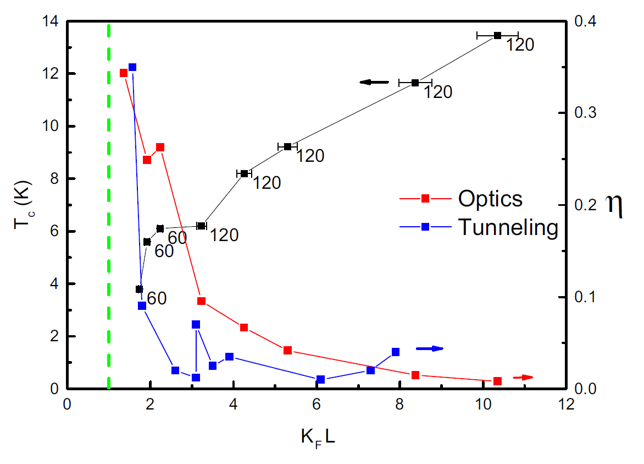
\includegraphics[width=0.49\textwidth]{T_c_disoreder_dependence.png}
	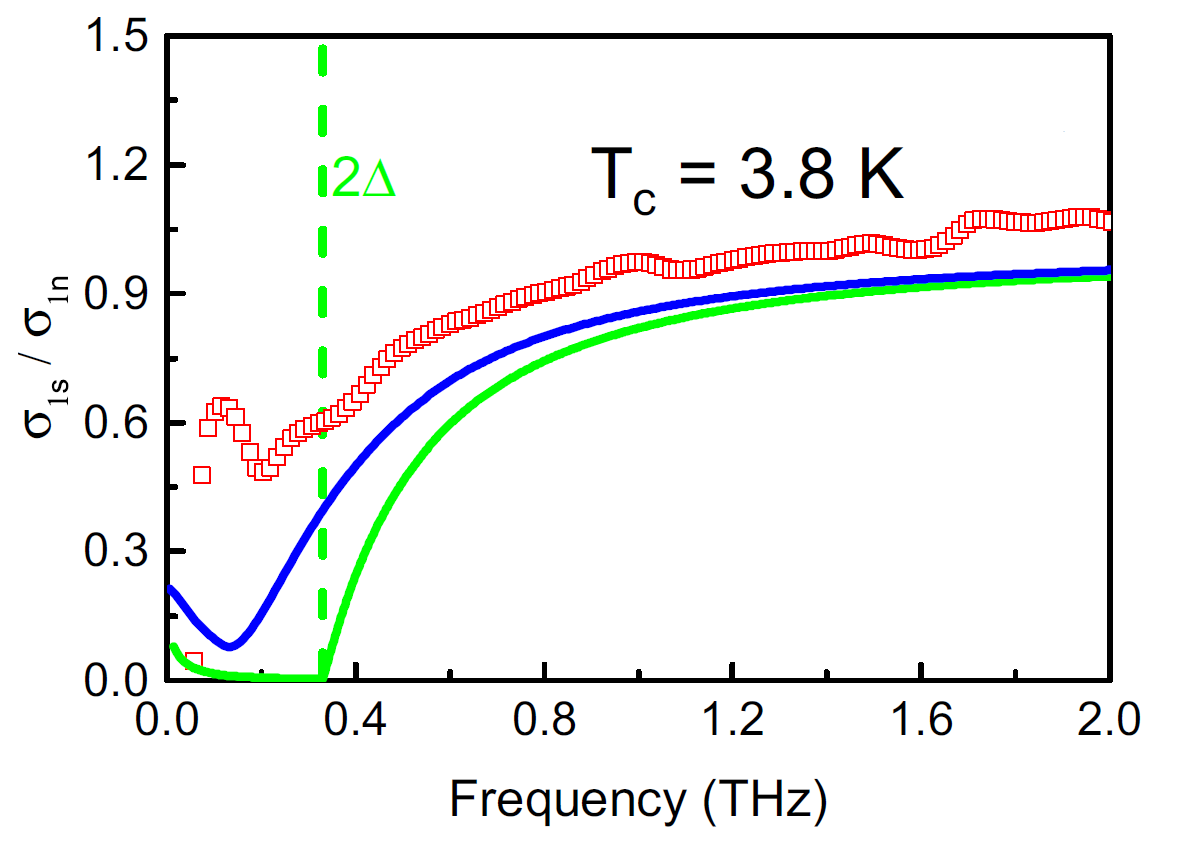
\includegraphics[width=0.4\textwidth]{Real_conductivity_frequency_dependence.png}
	\caption{Демонстрация влияния сильного беспорядка на ключевые свойства сверхпроводимости на примере плёнок NbN. Слева, чёрные символы: зависимость температуры сверхпроводящего перехода от степени загрязнения металла, измеряемой безразмерным параметром $k_F l$, где $k_F$ --- импульс Ферми, а $l$ -- длина свободного пробега. Параметр $k_F l$ определялся по сопротивлению при комнатной температуре. Данные взяты из работы \cite{Cheng_2016}. Справа, красные символы: зависимость действительной части проводимости металла от частоты внешнего излучения. Зелёной линией отмечено положение сверхпроводящей щели, найденное средствами туннельной микроскопии. Данные также взяты из работы \cite{Cheng_2016}.}	
\end{figure}
Выборка из экспериментальных данных, более детально демонстрирующих обсуждаемые эффекты на примере плёнок NbN, приведена на Рис. \ref{fig:Impur_Tc_and_radiation_absorb_data}. Существенно, что обсуждаемые эффекты происходят в макроскопически однородных образцах, где характерные масштабы неоднородностей существенно микроскопические. В частности, беспорядок в плёнках NbN создаётся за счёт вакансий Nb в кристаллической решётке \cite{Cheng_2016}. Схожими свойствами обладают также и ряд других образцов:
\begin{itemize} 
	\item плёнки InO, в которых также наблюдались описываемые явления \cite{Sherman_2015}, и беспорядок в которых имеет стехиометрическую природу, т. е. задаётся аморфной структурой вещества;
	\item плёнки из наногранул Al \cite{Pracht_2016}, в которых микроскопические неоднородности задаются непосредственно структурой из гранул алюминия размерами $\sim 2 nm$, разделённых оксидной плёнкой. В этом случае микроскопичность неоднородностей проявляется в том, что отдельно взятая гранула в силу своих малых размеров не обладает достаточными числом состояний для развития сверхпроводящих эффектов.
\end{itemize}

Эффект изменения температуры перехода $T_c$ в макроскопически однородных загрязнённых образцах уже получил теоретическое описание \cite{Feigelman2010}, и качественно объясняется влиянием эффектов Андерсоновской локализации и преформирования Куперовских пар (несколько подробнее эта эффекты мы разберём далее). Однако этого нельзя сказать о факте наличия низкоэнергетических возбуждений: существует лишь ряд эмпирических теорий, не дающих объяснения природе наблюдаемого явления (см., опять же, \cite{Cheng_2016}, \cite{Sherman_2015}). В данной работе будет произведена попытка разработать количественную микроскопическую модель, описывающую низкоэнергетические возбуждения в грязном сверхпроводнике. Теоретическое описание будет строиться на основе идей, развитых в \cite{Feigelman2010}, а также в значительной степени будет опираться на изложенные в работе \cite{FI_microwave} гипотезы по конкретной реализации упомянутой модели.



\section{Схема организации работы}
Данная работа организована следующим образом:
\begin{itemize}
	\item в \autoref{Theor}, посвящённой непосредственно теоретическому описанию явления низкоэнергетических возбуждений, будет дано подробное описание модельной задачи, предположительно содержащей ключевые эффекты.
	\begin{itemize}
		\item Сначала представлено феноменологическое введение, мотивирующее последующие упрощающие предположения. По итогу будет выписан т. н. псевдоспиновый гамильтониан на $K$-регулярном графе, использующийся далее для описания всей физики <<грязной>> сверхпроводимости.
		\item На его основе с помощью формализма семионного представления Попова-Федотова будут выведены основные уравнения, описывающее сверхпроводящее состояние: уравнение самосогласования и квадратичная часть функционала Гинзбурга-Ландау.
		\item Наконец, построенный формализм позволит поставить задачу, непосредственно описывающую в рамках данной модели низкоэнергетические возбуждения в сверхпроводнике. 
		\item Последним пунктом будут изложены упрощения, позволяющие решить поставленную задачу в терминах локальной плотности состояний некоторого линейного оператора на $K$-регулярном графе. Будут также приведены имеющиеся теоретические предсказания, связанные с этой упрощённой моделью.
	\end{itemize}

	\item в \autoref{Numer} будет подробно изложена теория метода популяционной динамики, предоставляющего способ численного решения поставленной в конце \autoref{Theor} упрощённой задачи.
	\begin{itemize}
		\item Для начала будет приведено введение в теорию, позволяющую установить соответствие между задачами на больших регулярных графах и на древесных графах с постоянным ветвлением.
		\item Далее будет приведён вывод и подробное описание алгоритма популяционной динамики вкупе с проделанными оптимизациями. Будет также установлена связь изучаемых величин с задачей локализации Андерсона с диагональным беспорядком.
		\item Затем будут приведено сравнение алгоритма с уже имеющимся методом исследования схожих задач и разобраны основные особенности поведения данной численной процедуры.
	\end{itemize}

	\item \autoref{Result} представит читателю обзор результатов численного исследования модели, физическую интерпретацию полученных сведений и вывода по дальнейшему изучению.
	\begin{itemize}
		\item Будут представлены подробные результаты, описывающие все важные аспекты статистики локальной плотности состояний упомянутого оператора. 
		\item Для основных характеристик статистики будет приведены имеющиеся численные данные, описывающие зависимости от параметра $K$.
		\item Полученные результаты будут интерпретированы с позиции уже известной теории задачи Андерсона. Будет представлен анализ сделанных ранее качественных и количественных предсказаний касательно этой модели.
		\item Наконец, будет представлена интерпретация полученных результатов в терминах исходной задачи описания низкоэнергетических возбуждений сверхпроводника и намечен план дальнейших исследований.
	\end{itemize}

	\item В финальной \autoref{Concl} приводится краткий обзор проделанной работы и резюмируются сделанные в процессе выводы.
\end{itemize}
%TODO: WRITE a paragraph about notations
% contraction rules, Heaviside function, Pauli matricies, E_F, k_F, l, \tau (Matrsubara imaginary time), \beta = 1/T, 